% Chapter Template

\chapter{Introduction} % Main chapter title

\label{Chapter1} % Change X to a consecutive number; for referencing this chapter elsewhere, use \ref{ChapterX}

% Define some commands to keep the formatting separated from the content 
\newcommand{\keyword}[1]{\textbf{#1}}
\newcommand{\tabhead}[1]{\textbf{#1}}
\newcommand{\code}[1]{\texttt{#1}}
\newcommand{\file}[1]{\texttt{\bfseries#1}}
\newcommand{\option}[1]{\texttt{\itshape#1}}

How the brain uses sensory information to guide decisions and actions remains an open question in systems neuroscience. One of the frameworks for studying the proposed question is perceptual decision making, or how subjects use sensory information to make decisions. This framework resides between low-level reflexive decision, which are characterized by sensory driven, involuntary impulses (e.g. pulling my hand away from a burning stove), and high-level cognitive decisions, which are characterized by voluntary choice largely independent of sensory information (e.g. do we have free will?) The perceptual decision making framework emphasizes the gathering and utilization of available sensory information to make choices between competing outcomes. Typically, such decisions involve categorical judgments about the nature or identity of sensory stimuli \parencite{Ding2013}. For example, is the car in my rearview mirror approaching too fast and should I change lanes? \par 

Perceptual decisions are made across modalities and space and are integrated with prior experiences. They often also require deliberation or the accumulation of sensory evidence over time. In this accumulation framework, the subject gradually gathers sensory information in favor of or against competing choices. The brain computes a decision variable based on the available evidence, which is compared against a decision boundary and ultimately the subject makes a choice. Where and how the brain accumulates this evidence and classifies it according to a decision boundary is the subject of intense research across multiple model organisms. In this chapter, I summarize this research including the seminal studies in non-human primates and recent work from rodents. 

\section{Evidence Accumulation: Non-human primate studies}
The random dots kinectogram task has been a staple in perceptual decision making studies investigating accumulation of sensory evidence. In the task, the subject makes a categorical decision about global direction of motion of randomly moving dots on a monitor display. The task difficulty is controlled by varying the fraction of dots coherently moving in one direction. The easiest trials have a high proportion of dots moving coherently (high coherence), and more difficult trials have a small proportion of dots that move coherently (low coherence). The goal of the subject is to discriminate the global direction (eg. left vs. right) of the dots stimulus. Rhesus macaques are trained to indicate decisions by saccadic eye movements toward the direction of the coherent motion \parencite{Britten1992}.\par 

Physiological measurements and causal manipulation experiments in macaque subjects performing the dots task revealed that the moment by moment representation of motion evidence is encoded in the activity of extrastriate visual area MT (middle temporal or area V5) \parencite{Albright1984,Newsome1988,Salzman1992}. The presence of the random dots stimuli elicits sustained responses in MT, which scale linearly with the motion evidence \parencite{Britten1993}. \par 

The noisy nature of the dots stimulus invites the subject to integrate the evidence over time to optimize decisions. One plausible way for the brain to read out the momentary evidence from area MT is to integrate. Here, the integral of the motion evidence represents the internal decision variable used to make a categorical decision. Neural recordings from several brain areas exhibit ramp-like neural activity patterns during the decision process consistent with the integral of motion evidence, and thus plausible accumulation of evidence process. In particular, neural responses in the lateral intra-parietal (LIP) area of the posterior parietal cortex (PPC) reflected integration of evidence  \parencite{Shadlen1996,Hanes1996,Shadlen2001}. In primates and humans, PPC plays a central role in processing of visual information for guiding actions.   Further, neural correlates of evidence integration have also been observed in several other brain areas including the superior colliculus (SC), dorsolateral prefontal cortex (dlPFC), frontal eye field (FEF), and the striatum \parencite{Horwitz1999,Horwitz2001,Kim1999,Purcell2010,Ding2012,,Mante2013,Ding2010}.\par 

Interestingly, area LIP is interconnected with each of these brain areas (Table \ref{table:areaLIP}) \parencite{Cavada1989a,Cavada1989c,Cavada1991}, suggesting that the accumulation of evidence process might be a distributed process involving multiple brain regions in concert. Recent evidence in support of this view comes from a study from \parencite{Katz2016}. The authors found that selective inactivation of area LIP during the random dots task had negligible effect on the behavior. This finding is in contrast to experiments in which microstimulation of area LIP biased choices and reaction time of macaque subjects performing the random dots task \parencite{Hanks2006}. The LIP inactivation result is not surprising if one assumes that a distributed network of brain areas reflect the evidence accumulation process. These areas may compensate for the loss of LIP activity while similarly, the addition of aberrant microstimulation signal would disrupt performance because the brain regions are interconnected.\par 
\begin{figure}
\centering
  	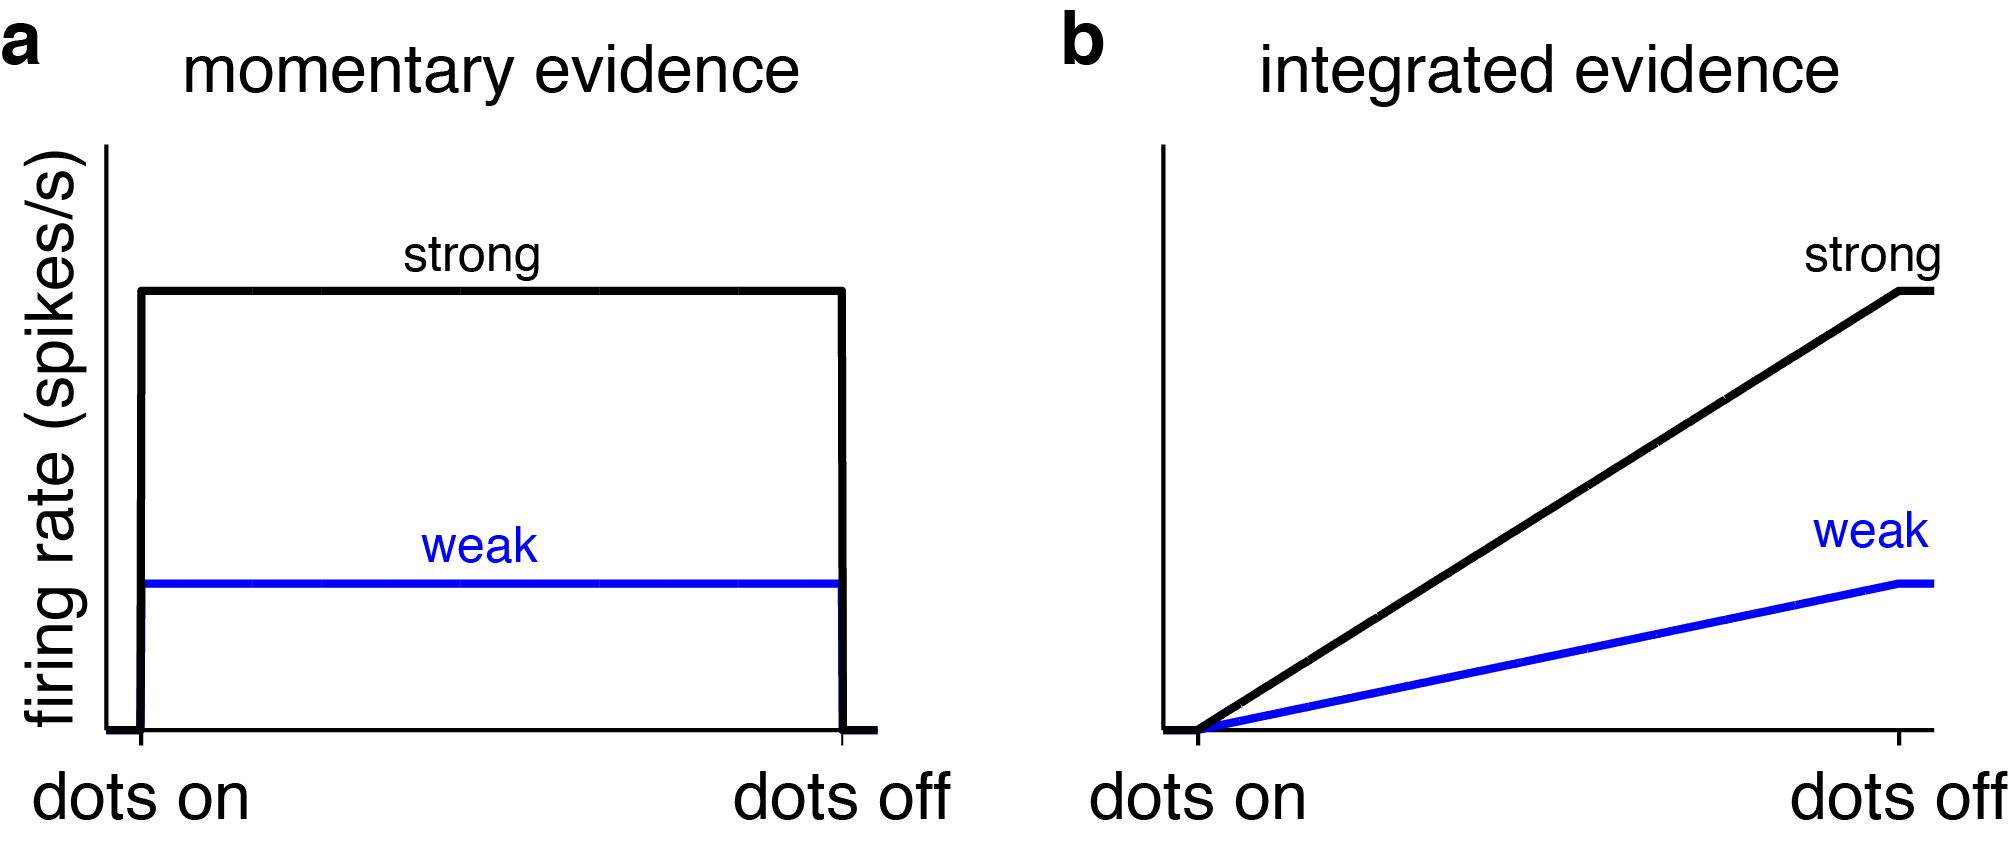
\includegraphics[scale=0.6]{Figures/chapter1/area_MT_LIP_activity_schematic.png}
  \caption[Schematic of Motion Evidence in MT and Integrated Evidence]{\textbf{Schematic of Motion Evidence in MT and Integrated Evidence} The integral (cumulative sum) of the momentary evidence is a ramp-like function reflecting the decision variable. Weak evidence in blue and strong evidence in black.}
   \label{fig:schematic}
\end{figure}
In summary, the standard model proposed by evidence accumulation studies in macaque subjects is that momentary evidence is encoded in area MT (Figure \ref{fig:schematic} a) and the decision variable or integrated evidence is reflected in multiple brain areas including LIP, SC, dlPFC, FEF, and striatum (Figure \ref{fig:schematic} b). Several open questions still remain: for instance, which of the candidate areas reflecting the accumulated evidence are critical to the decision process? How is the accumulation of evidence process implemented? What circuit architecture supports the sensory integration over time? Is the integration of evidence strictly computed by dedicated neurons/areas or is it an emergent property of distributed processing of sensory information?

\section{Evidence Accumulation: Rodent studies}
Addressing these open questions has been challenging in nonhuman primate subjects largely due to the cost and technical constraints. As a result, many scientists have turned to rodents as a complementary model organism for studying the neural circuit mechanism of evidence accumulation. Rodents offer a wide variety of tools for measuring and manipulating neural activity with cell-type specificity. Rodents share a common mammalian ancestor with primates dating back 75-100 million years ago \parencite{Murphy2004} and both species belong to the mammalian superorder \emph{Euarchontoglires}. They possess many of the same brain areas and general brain organization found in primates and humans \parencite{Kaas2009}. The smooth, lissencephalic cortex of rodents is an advantage because brain areas are easily accessible for electrical and optical neural recordings. Rodents also occupy a smaller footprint compared to macaques, and therefore are readily amenable to large-scale studies using numerous subjects. \par 

Although rodents have been trained to perform decision tasks with the random dots stimulus \parencite{Douglas2006,Reinagel2013,Petruno2013,Stirman2016}, recent evidence accumulation studies have introduced discrete pulsatile stimulus sequences. The main advantage of the discrete pulse stimulus is that the evidence at each moment of time and on each trial is known, which is useful when modeling the accumulator value on each trial \parencite{Brunton2013,Hanks2015}. This thesis will focus on tasks using discrete pulsatile sequences.

\subsection{Rats}
Building on the non-humnan primate work in evidence accumulation, several behavioral paradigms have been developed in the rat towards the goal of understanding the neural mechanisms underlying evidence accumulation. \textcite{Raposo2012a} developed a multisensory decision task in which rats were presented with a random sequence of auditory clicks, visual flashes, or both modalities and the rats learned to make a categorical judgment about whether rate of sensory events exceeded a decision boundary. In a parallel study by \textcite{Brunton2013}, rats were presented with two spatially-separate streams of auditory 'Poisson' clicks and learned to make a categorical judgment as to which of the two streams contained more clicks. The same group also developed a separate visual modality version of the 'Poisson' clicks task \parencite{Scott2015SourcesRats}. A third group developed an auditory analog of the random dots task referred to as the 'cloud of tones' task \parencite{Znamenskiy2013b}. In the task, rats judged whether a series ("cloud") of overlapping tones consisted of high-frequency vs. low-frequency tones. \par 

Neural recordings from the rat PPC, at first glance, are consistent with evidence accumulation signatures observed in primate LIP. For example, the firing rates of the neurons in rat PPC exhibit ramp-like activity proportional to the evidence strength \parencite{Raposo2014,Hanks2015}. However, closer inspection of the activity in rat PPC reveal that sensory evidence in accumulated elsewhere \parencite{Hanks2015} and that rat PPC might instead play a role in visual processing \parencite{Licata2017}. Observations from causal manipulation of rat PPC are consistent with the neuropphysiological measurements. Rat PPC activity is not required for performing auditory evidence accumulation \parencite{Raposo2014,Erlich2015}, but it is required for visual evidence accumulation \parencite{Raposo2014,Licata2017}. 

\subsection{Mice}
Mice are an ideal model system for studying neural circuits because of the abundant tools for accessing and probing genetically defined cell types \parencite{Madisen2010,Taniguchi2011,Madisen2012,Madisen2015}. However, in contrast to rats, mice are largely underrepresented in evidence accumulation paradigms, even though mice can be trained to achieve similar levels of performance as rats in perceptual decision-making paradigms \parencite{Douglas2006,Jaramillo2014}. A literature search at the beginning of my thesis research for evidence accumulation tasks in mice yielded only a handful of studies \parencite{Douglas2006,Sanders2012}. \textcite{Douglas2006} trained mice (and rats) to report the direction of random dots by swimming towards a target. This paradigm is not scalable for large cohorts of mice and limits the options for measuring neural activity \emph{in vivo} in behaving animals. In the task developed by \textcite{Sanders2012}, head-fixed mice were trained to report decisions by moving a ball with their paws to the left or the right, depending on which spatial location produced more random pulsatile auditory clicks. This task is well suited for neural measurements, but it is not clear whether large numbers of mice can be trained to successfully perform the task. \par 

Recently, parallel to the work presented in this thesis, several mouse evidence accumulation tasks have emerged \parencite{Stirman2016,Marcos2016,Marbach2016}, reflecting the growing interest in leveraging the benefits of the mouse model for studying neural circuits underlying evidence accumulation. To be clear, I am referring to tasks in which mice are presented with stimuli that vary stochastically across time and therefore require temporal integration (accumulation) of the stimulus to make accurate decisions. Several authors have successfully trained mice on a variety of sensory perception tasks that do not require temporal accumulation of evidence including: 
\parencite{Andermann2010a,Busse2011,Glickfeld2013b,Jaramillo2014,Guo2014b,Burgess2016,Jeong2017}.\par 

It is not established whether mice performing an evidence accumulation task perform as well as the rats trained on the same task or whether mice use the same strategy and/or neural machinery to solve such a task. This thesis will address some of these issues in subsequent chapters. 

% \section{Anatomy of Visual and Parietal Cortices}
% \subsection{Primates}
\section{Definition of Mouse Posterior Parietal Cortex}
PPC is an anatomical region located between somatosensory and visual areas in cortex. It receives inputs from these sensory cortices and projects to frontal motor areas; thus PPC sits at the interface of sensory and motor systems \parencite{Andersen2002}. In primates and humans, this area is greatly expanded and consists of multiple anatomically \parencite{Cavada2001,Cavada1993} and functionally distinct subdivisions \parencite{Andersen2002,Kaas2016} specialized for different actions. Area LIP, discussed previously, is among these PPC subdivisions.\par 

In rodents, the equivalent area referred to as PPC is very narrow strip between primary somatosensory (S1) and visual cortex (V1). Given the relatively small size of the rodent brain and the limited cortical real estate within this strip, it is unclear whether rodents possess a dedicated PPC area. Furthermore, in the mouse, several distinct retinotopic visual areas \parencite{Wang2007} (Figure \ref{fig:vis_areas}a) have been found to reside within the narrow strip. It is not known whether the same is true for the rat, which also have multiple visual areas that surround V1\parencite{Montero1973a,Espinoza1983}. \par 

The most commonly used definition for mouse PPC originates from \textcite{Harvey2012}. Here, PPC was defined based on anatomical projections from an area anterior to primary visual cortex (V1) and posterior to primary somatosensory cortex (S1). Although the anatomical connectivity patterns of their mouse PPC area (Table \ref{table:harveyPPC} ) are similar to those found in nonhuman primate area LIP (Table \ref{table:areaLIP}), the areal extent or boundary of the Harvey et al mouse PPC is not defined, nor is it established whether mouse PPC overlaps with multiple subdivisions as has been observed in primates and rats.\par 

An intriguing hypothesis is that mouse PPC is one or more higher-order visual areas which represent the ancestral (or evolutionary) precursors to PPC found in primates. Candidate higher-order visual areas in the anatomical region between V1 and S1 that qualify as an equivalent PPC area, or subdivision thereof, include areas RL, A, AM, MMA, and RLL. With the exception of MMA and RLL, which were recently discovered \parencite{Zhuang2017}, these areas posses distinct connectivity patterns (input and output) and functional responses to features of grating stimuli \parencite{Andermann2011,Marshel2011,Juavinett2015,Tohmi2014}. These areas also project to frontal motor areas \parencite{Wang2012}, a hallmark feature of sensorimotor areas like PPC \parencite{Kaas2011a}. Furthermore, the functional roles of these higher visual areas in behavior remain unknown. \par

%table generated with http://www.tablesgenerator.com/
\begin{table}
\centering
\begin{tabular}{cl}
\hline
\multicolumn{2}{c}{Areas} \\ \hline
\textbf{Visual} & V1,V2 \\
\textbf{Motor} & M2 \\
\textbf{Frontal} & mPFC, Orbitofrontal \\
\textbf{Limbic} & Cingulate, Retrosplenial, Perirhinal \\
\textbf{Subcortical} & Striatum, Superior Colliculus \\ \hline
\end{tabular}
\caption[Stereotactic Mouse PPC Connectivity Summary]{\textbf{Stereotactic Mouse PPC Connectivity Summary} Anatomical connectivity pattern of mouse PPC defined by \textcite{Harvey2012}.}
\label{table:harveyPPC}
\end{table}

\begin{table}
\centering
\begin{tabular}{cl}
\hline
\multicolumn{2}{c}{Areas} \\ \hline
\textbf{Visual} & \begin{tabular}[c]{@{}l@{}}MT, FST, STP, IT, V2, \\ V3, V4, PO\end{tabular} \\
\textbf{Motor} & FEF, Premotor \\
\textbf{Frontal} & Prefontal Cortex, Orbitofrontal \\
\textbf{Limbic} & \begin{tabular}[c]{@{}l@{}}Cingulate, Retrosplenial,\\ Presubiculum, Perirhinal\end{tabular} \\
\textbf{Subcortical} & Striatum, Superior Colliculus, Pons \\ \hline
\end{tabular}
\caption[Area LIP Projections Summary]{\textbf{Area LIP Projections Summary} Cortical and Subcortical projections from area LIP \parencite{Cavada1989a,Cavada1989c,Cavada2001} MT, medial temporal area; FST, fundal superior temporal area; STP, superior temporal polysensory area; IT, inferior temporal cortex; V2, visual area 2; V3, visual area 3; V4, visual area 4; PO, parieto-occipital area; FEF, frontal eye field.}
\label{table:areaLIP}
\end{table}

%------------------------------------------------------------------
\begin{figure}
\centering
  	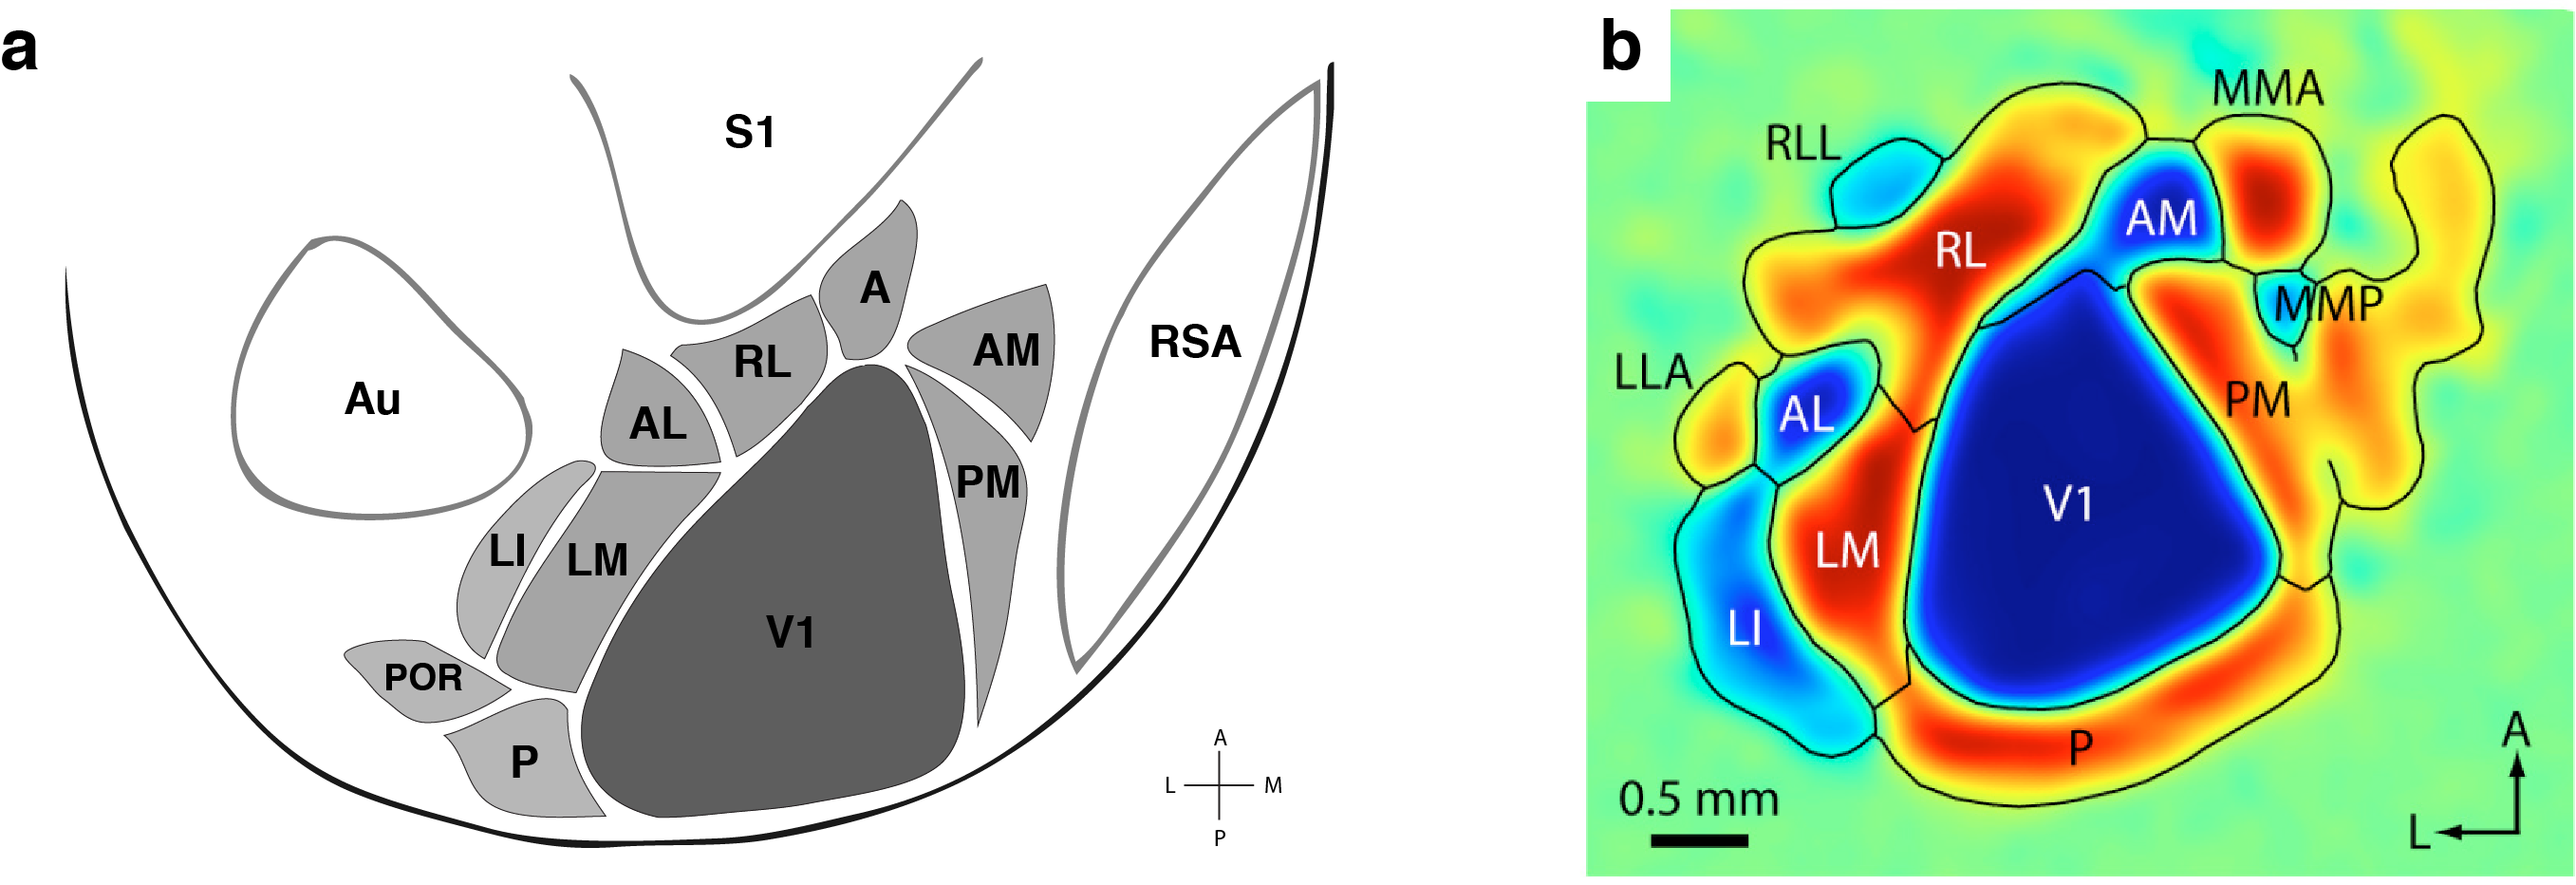
\includegraphics[width=\textwidth]{Figures/chapter1/visual_areas_map.png}
  \caption[Mouse Visual Cortex and the Surrounding Areas]{\textbf{Mouse Visual Cortex and the Surrounding Areas} (a) Schematic of the original nine secondary visual areas identified by \textcite{Wang2007} in light gray. (b) The extended retinotopic map based on widefield calcium imaging by \textcite{Zhuang2017} includes additional areas not present in the original map (a).} 
   \label{fig:vis_areas}
\end{figure}

\section{Thesis Outline}
Due to the vast genetic tools available, mice are currently a superior model organism for casual studies examining the role of brain areas and neural activity in the accumulation of sensory evidence and production of behavior. However, the usefulness of mice in studies of perceptual decision making, and in particular evidence accumulation, is limited by current lack of knowledge concerning whether mice can learn accumulation tasks and the anatomy/connectivity of mouse sensory and decision making areas. This thesis aims to address this paucity of knowledge. \par 

In Chapter \ref{Chapter2}, I describe the psychophysical paradigm for investigating evidence accumulation in mice and provides quantitative description of the mouse behavior. In Chapter \ref{Chapter3}, I describe causal manipulation experiments of mouse PPC defined by stereotactic coordinates provided by \textcite{Harvey2012} in order to address the role for a putative mouse PPC homologue in evidence accumulation. In Chapter \ref{Chapter4}, I discuss experiments aimed at targeting a secondary visual area and putative subdivision of mouse PPC, area AM, for inactivation during visual evidence accumulation. Finally, in Chapter \ref{Chapter5}, I discuss results of analyses that reveal insights about how mice process natural scene images, forming the basis for an understanding of how mice may use sensory information to guide decisions.

